\documentclass[xcolor=dvipsnames]{beamer}
\usetheme{Madrid}

\usepackage[italian]{babel}

\usepackage[utf8]{inputenc}

\usepackage{hyperref}
\usepackage{graphicx} % Allows including images
\usepackage{booktabs} % Allows the 

\newcommand{\R}{\mathbb{R}}
\newcommand{\C}{\mathbb{C}}
\newcommand{\Z}{\mathbb{Z}}
\newcommand{\mc}[1]{\mathcal{#1}}
\newcommand{\ii}[1]{\textit{#1}}
\newcommand{\req}[1]{\stackrel{#1}{=}}
\newcommand{\bra}[1]{\langle #1 |}
\newcommand{\ket}[1]{| #1 \rangle}
\newcommand{\braket}[2]{\langle #1 | #2 \rangle}

\title{Geometric Deep Learning}
% \author{Tommaso Lamma}
\date{17 settembre 2021}

\begin{document}

\frame{\titlepage}

\frame{\tableofcontents}

\section{Reti Convoluzionali}

\begin{frame}
    \frametitle{Reti Convoluzionali}
    \begin{figure}[H]
        \centering
        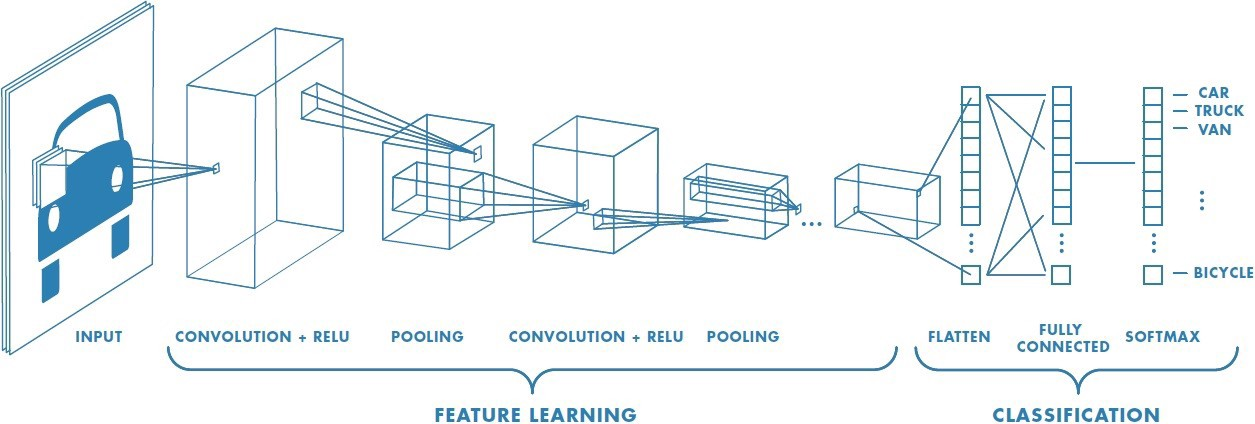
\includegraphics[width=10cm, height=4cm]{cnn}
        \caption{Una rete neurale convoluzionale.}
    \end{figure}       
\end{frame}

\section{Convoluzione su Domini Euclidei}

\begin{frame}
    \frametitle{Convoluzione su Domini Euclidei}    
    Siano $f:\R \to \R$ e $g:\R \to \R$,
    \[ (f * g)(x) = \int_{\R} dx' f(x')g(x-x'). \]
    \hfill \\
    \hfill \\
    { \large Cosa significa $(x - x')$ in un dominio diverso da $\R$ ?}
\end{frame}

\begin{frame}
    \frametitle{ \large Cosa significa $(x - x')$ \textbf{in} $\R$ ?}
    \hfill \\
    \hfill \\
    \begin{block}{Notare:}
        Il gruppo $(\R, +)$ è una simmetria globale del dominio $\R$.  
    \end{block}
    \hfill \\
    \hfill \\
    {\large Possiamo definire una convoluzione a partire da una simmetria?}
\end{frame}

\begin{frame}
    \frametitle{Impostazione del problema}
    \begin{block}{Operatore Posizione}
        \[ \widehat{x}|x\rangle = x | x \rangle \quad x \in \R \]
        \[ \langle x | x' \rangle = \delta(x-x'), \quad
    \int_{\R} dx | x \rangle \langle x | = \widehat{1} .\]
    \end{block}
    \begin{block}{Operatore Impulso}
    \[ \widehat{p} | p \rangle = p | p \rangle, \]
    \[ \langle p | p' \rangle = \delta(p-p'), \quad
    \int_{\R} dp | p \rangle \langle p | = \widehat{1} .\]
    \end{block}
    L'operatore $\widehat{p}$ genera le traslazioni
        \[ \langle x | e^{-i \widehat{p} x'} | p \rangle = \langle x | p \rangle \langle -x' | p \rangle \sqrt{2 \pi} = \langle x-x' | p \rangle, \]
        \[ \langle x | e^{-i \widehat{p} x'} = \langle x-x' | .  \]
\end{frame}

\begin{frame}
    \frametitle{Teorema della Convoluzione}
    \begin{block}{Trasformata di Fourier}
        \[ \langle p | \psi \rangle = \langle p | \left( \int_{\R} dx | x \rangle \langle x| \right) | \psi \rangle = 
         \int_{\R} dx \langle p | x \rangle \langle x | \psi \rangle. \]
    \end{block}
    Dove $\langle x | p \rangle = \frac{e^{ipx}}{\sqrt{2 \pi} }$ e $\langle x | \psi \rangle := \psi(x) $.
    \begin{block}{Teorema della Convoluzione}
        \[ \langle p | \psi * \phi \rangle = \sqrt{2\pi} \langle p | \psi \rangle \langle p | \phi \rangle . \]
    \end{block}
   \[ \widehat{C}_\phi | \psi \rangle  := | \psi * \phi \rangle . \]
    Il teorema della convoluzione piò essere visto come
    \[ \langle p | \psi * \phi \rangle =: \langle p | \widehat{C}_\phi |\psi \rangle = \sqrt{2\pi} \langle p | \psi \rangle \langle p | \phi \rangle \]
   \[ {\color{blue} \langle p | \widehat{C}_\phi = \sqrt{2\pi} \langle p | \psi \rangle \langle p | }\]
\end{frame}

\begin{frame}
    \frametitle{Definizione di Convoluzione}
    \begin{block}{Definizione di Convoluzione}
        \[ \widehat{C}_\phi = \sqrt{2\pi} \int_\R dp | p \rangle \langle p | \phi \rangle \langle p | . \]
    \end{block}
    \begin{block}{Convoluzione $\R$-Equivariante}
        \Large
        \[ [ \widehat{p}, \widehat{C}_\phi] = 0 .\]
    \end{block}
\end{frame}

\begin{frame}
    \frametitle{Recuperiamo l'altra definizione}
     \[ \langle x | \widehat{C}_\phi | \psi \rangle = \sqrt{2\pi} \int_\R dp \langle x | p \rangle \langle p | \phi \rangle \langle p | \psi \rangle = \] \[
      = \sqrt{2\pi} \int_\R dx' \int_\R dy \left( \int_\R dp \langle x | p \rangle \langle p | x' \rangle \langle p | y \rangle \right) \langle x' | \phi \rangle 
     \langle y | \psi \rangle = \] \[ =  \sqrt{2\pi} \int_\R dx' \int_\R dy \frac{\delta(x - x' - y)}{\sqrt{2\pi}} \langle x' | \phi \rangle \langle y | \psi \rangle = 
     \int_\R dx' \langle x - x' | \phi \rangle \langle x' | \psi \rangle . \]
     Da cui
     {\color{blue}\[ \langle x | \psi * \phi \rangle = \int_\R dx' \langle x - x' | \phi \rangle \langle x' | \psi \rangle. \] }  
\end{frame}

\section{Convoluzione su Domini \textbf{non} Euclidei}

\begin{frame}
    \frametitle{Convoluzione su Domini non Euclidei}
    \begin{figure}[H]
        \centering
        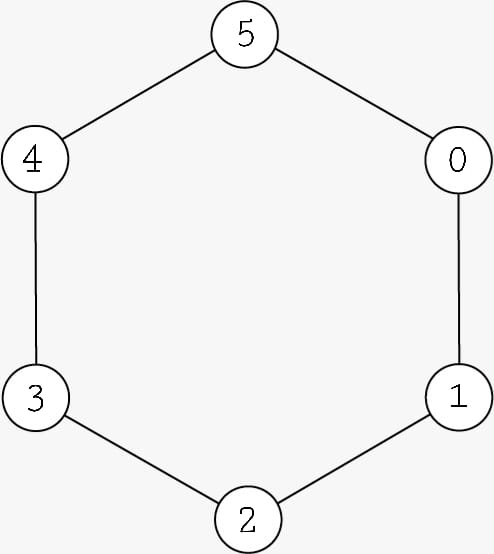
\includegraphics[width=5cm, height=5cm]{graph}
        \caption{Un dominio non euclideo $\mc{G}$.}
    \end{figure}    
\end{frame}

\begin{frame}
    \frametitle{Impostazione del problema}
    \begin{block}{Operatore Posizione}
        \[ \widehat{x}|i\rangle = i | i \rangle \quad i \in C_0 \]
        \[ \langle i | j \rangle = \delta_{ij}, \quad
    \sum_{i \in \Z_6} | i \rangle \langle i | = \widehat{1} .\]
    \end{block}
    \begin{block}{Operatore impulso che genera $\Z_6$}
    \[  \langle i | \widehat{S}  = \langle i+1 |, \]
    \end{block}
\end{frame}

\begin{frame}
    \begin{block}{Azione del generatore sulle componenti}
        \[ \langle i | \widehat{S} | \psi \rangle =  \sum_{j \in \Z_6} \langle i+1 | j \rangle \langle j | \psi \rangle = \psi_{i+1} = \langle i+1 | \psi \rangle, \]
        dove $ \langle i | \widehat{S} | j \rangle = \langle i+1 | j \rangle = circ(0,1,0,0,0,0) =: \begin{pmatrix} 0 & 1 & 0 & 0 & 0 & 0 \\ 0 & 0 & 1 & 0 & 0 & 0 \\ 0 & 0 & 0 & 1 & 0 & 0
        \\ 0 & 0 & 0 & 0 & 1 & 0 \\ 0 & 0 & 0 & 0 & 0 & 1 \\ 1 & 0 & 0 & 0 & 0 & 0 \\ 
    \end{pmatrix}$.
    \end{block}  
    L'operatore $\widehat{S}$ è diagonalizzabile in $\C$ con una base \textbf{ortonormale} \[ \widehat{S}|s_i \rangle = s_i | s_i \rangle, \]
    \[ \langle s_i | s_j \rangle = \delta_{ij}, \quad
    \sum_{i \in \Z_6} | s_i \rangle \langle s_i | = \widehat{1} .\]  
\end{frame}

\begin{frame}
    \frametitle{Teorema della Convoluzione}
    \begin{block}{Trasformata di Fourier}
        \[ \langle s_i | \psi \rangle = \langle s_i | \left( \sum_{j \in \Z_6} | j \rangle \langle j| \right) | \psi \rangle = 
        \sum_{j \in \Z_6} \langle s_i| j \rangle \langle j | \psi \rangle. \]
    \end{block}
    \begin{block}{Teorema della Convoluzione}
        \[ \langle s_i | \psi * \phi \rangle = \langle s_i | \psi \rangle \langle s_i | \phi \rangle . \]
    \end{block}
    \[ \widehat{C}_\phi | \psi \rangle  := | \psi * \phi \rangle . \]
    Il teorema della convoluzione piò essere visto come
    \[ \langle s_i | \psi * \phi \rangle =: \langle s_i | \widehat{C}_\phi |\psi \rangle =\langle s_i | \psi \rangle \langle s_i | \phi \rangle \]
   \[ {\color{blue} \langle s_i | \widehat{C}_\phi = \langle s_i | \psi \rangle \langle s_i | }\]
\end{frame}

\begin{frame}
    \frametitle{Definizione di Convoluzione}
    \begin{block}{Definizione di Convoluzione}
        \[\widehat{C}_\phi = \sum_{j \in \Z_6} | s_j \rangle \langle s_j | \phi \rangle \langle s_j |.\]
    \end{block} 
    \begin{block}{Convoluzione $\Z_6$-Equivariante}
        \Large
        \[ [ \widehat{S}, \widehat{C}_\phi] = 0 .\]
    \end{block}
\end{frame}

\begin{frame}
    \frametitle{Un'Altra Simmetria}
    \begin{block}{Equazione del Calore}
        \[ \frac{d}{dt} | \psi \rangle = -\widehat{\Delta} | \psi \rangle , \]
        dove $\widehat{\Delta} = \text{diag}(\text{deg}(i))-A$.
    \end{block}
    \begin{block}{Convoluzione Equivariante Rispetto alla Diffusione}
        \[ \widehat{C}_\phi = \sum_{i = 1}^{\text{dim} C_0} | e_i \rangle \langle e_i | \phi \rangle \langle e_i |,  \]
        dove $\widehat{\Delta} | e_i \rangle = \lambda_i | e_i \rangle $.
    \end{block}
\end{frame}

\section{Equivarianza}

\begin{frame}
    \frametitle{Equivarianza}
    \begin{block}{Simmetrie di una classificazione $ \mc{C} : \mc{S} \to \mc{L}$ }
       \[ \text{Sym}(\mc{C}) := \{ g : \mc{S} \to \mc{S} \; : \; \mc{C}(f) = \mc{C}(f \circ g) \; \forall f \in \mc{S} \} .\]
    \end{block}
    \begin{center}
    \Large $(\text{Sym}(\mc{C}), \circ)$ è un gruppo. 
    \end{center}
    % \begin{block}{Rete Convoluzionale Invariante}
    %     \[ \widehat{R} := \widehat{I} \left( \prod_i \widehat{E}_i \right)\]
    % \end{block}
\end{frame}

\begin{frame}
    \begin{center}
        \Huge
        Grazie per l'attenzione
    \end{center}
\end{frame}

\end{document}